\documentclass[11pt]{article}
\usepackage[margin=1in,top=1.1in,bottom=1.1in]{geometry}
\usepackage[utf8]{inputenc}
\usepackage[T1]{fontenc}
\usepackage{amsmath,amssymb,amsthm}
\usepackage{graphicx}
\usepackage{booktabs}
\usepackage{array}
\usepackage{makecell}
\usepackage{caption}
\usepackage{float}
\usepackage{placeins}
\usepackage{xcolor}
\usepackage{microtype}
\usepackage[colorlinks=true,linkcolor=blue,citecolor=blue,urlcolor=blue]{hyperref}

\captionsetup{font=small,labelfont=bf,width=0.95\textwidth}
\graphicspath{{figures/}{figures_supp/}}
\setlength{\emergencystretch}{4em}
% Auto-generated by tools/sync_crossrefs.py; do not edit manually.
\makeatletter
\newcommand{\MainRef}[1]{\csname MainRef@#1\endcsname}
\expandafter\newcommand\csname MainRef@eq:axis-agreement\endcsname{11}
\expandafter\newcommand\csname MainRef@eq:f-decomposition\endcsname{1}
\expandafter\newcommand\csname MainRef@eq:f-reduced\endcsname{2}
\expandafter\newcommand\csname MainRef@eq:m-centre\endcsname{5}
\expandafter\newcommand\csname MainRef@eq:m-coherent\endcsname{13}
\expandafter\newcommand\csname MainRef@eq:m-conditional\endcsname{9}
\expandafter\newcommand\csname MainRef@eq:m-fit\endcsname{6}
\expandafter\newcommand\csname MainRef@eq:m-null\endcsname{8}
\expandafter\newcommand\csname MainRef@eq:m-project\endcsname{3}
\expandafter\newcommand\csname MainRef@eq:m-roadbasis\endcsname{4}
\expandafter\newcommand\csname MainRef@eq:m-scores\endcsname{7}
\expandafter\newcommand\csname MainRef@eq:m-spectrum\endcsname{12}
\expandafter\newcommand\csname MainRef@eq:m-tensors\endcsname{10}
\expandafter\newcommand\csname MainRef@fig:concept\endcsname{1}
\expandafter\newcommand\csname MainRef@fig:road-tests\endcsname{5}
\expandafter\newcommand\csname MainRef@fig:threecity-evidence\endcsname{2}
\expandafter\newcommand\csname MainRef@fig:threecity-response\endcsname{4}
\expandafter\newcommand\csname MainRef@fig:threecity-spectrum\endcsname{3}
\expandafter\newcommand\csname MainRef@sec:comparison\endcsname{1.5}
\expandafter\newcommand\csname MainRef@sec:d-data\endcsname{3.1}
\expandafter\newcommand\csname MainRef@sec:disc\endcsname{2}
\expandafter\newcommand\csname MainRef@sec:formulation\endcsname{1.1}
\expandafter\newcommand\csname MainRef@sec:m-cons\endcsname{3.2}
\expandafter\newcommand\csname MainRef@sec:m-frames\endcsname{3.3}
\expandafter\newcommand\csname MainRef@sec:methods\endcsname{3}
\expandafter\newcommand\csname MainRef@sec:recon\endcsname{1.2}
\expandafter\newcommand\csname MainRef@sec:results\endcsname{1}
\expandafter\newcommand\csname MainRef@sec:spectra\endcsname{1.3}
\expandafter\newcommand\csname MainRef@sec:structure\endcsname{1.4}
\expandafter\newcommand\csname MainRef@tab:mainstream-main\endcsname{1}
\makeatother

\hypersetup{pdftitle={Supplementary Information -- Road-supported effective constitutive coupling and anisotropic routing responses in urban mobility},pdfauthor={Tiehang Xu, Jiahui Wang, Junyan Yang, Qiao Wang},pdfsubject={Supplementary Methods, Results and Reproducibility},pdfkeywords={urban mobility, Hodge decomposition, road networks, anisotropy}}
\newcommand{\repositorylocation}{\url{https://github.com/Wangwangw233/paper-urbanflow}}

% Notes, figures, tables and equations are rendered by counters, never typed numbers.
\newcounter{suppnote}
\renewcommand{\thesuppnote}{S\arabic{suppnote}}
\newcommand{\suppnote}[2]{%
  \FloatBarrier
  \refstepcounter{suppnote}%
  \subsection*{Note \thesuppnote\quad #1}%
  \label{#2}%
  \addcontentsline{toc}{subsection}{Note \thesuppnote\space #1}}
\newcommand{\suppsection}[1]{%
  \FloatBarrier\section*{#1}\addcontentsline{toc}{section}{#1}}

\renewcommand{\thefigure}{S\arabic{figure}}
\renewcommand{\thetable}{S\arabic{table}}
\renewcommand{\theequation}{S\arabic{equation}}

% --- notation ---------------------------------------------------------------
\providecommand{\R}{\mathbb{R}}
\providecommand{\rank}{\operatorname{rank}}
\providecommand{\tr}{\operatorname{tr}}
\providecommand{\argmin}{\operatorname*{arg\,min}}
\providecommand{\Fcirc}{F^{\circ}}
\providecommand{\Rcond}{R^{2}_{\mathrm{cond}}}
\providecommand{\UR}{U_{R}}
\providecommand{\CR}{C_{R}}
\providecommand{\Px}{P_{x}}
\providecommand{\SigC}{\Sigma_{C}}
\providecommand{\SigU}{\Sigma_{U}}
\providecommand{\AC}{A_{C}}
\providecommand{\AU}{A_{U}}
\providecommand{\Lc}{L_{c}}
\providecommand{\T}{\mathsf{T}}
\providecommand{\norm}[1]{\lVert #1 \rVert}

\title{Supplementary Information\\Road-supported effective constitutive coupling and anisotropic routing responses in urban mobility}
\author{Tiehang Xu$^{1}$ \and Jiahui Wang$^{2}$ \and Junyan Yang$^{3}$ \and Qiao Wang$^{1,2,\ast}$\\[0.5em]
\small
\begin{tabular}{@{}l@{}}
$^{1}$School of Information Science and Engineering, Southeast University, Nanjing, 210096, China\\
$^{2}$School of Economics and Management, Southeast University, Nanjing, 210096, China\\
$^{3}$School of Architecture, Southeast University, Nanjing, 210096, China\\
Emails: tiehangxu@seu.edu.cn; wangjh0521@seu.edu.cn; yjy-2@163.com; qiaowang@seu.edu.cn\\
$\ast$Correspondence: qiaowang@seu.edu.cn
\end{tabular}
}
\date{}

\begin{document}
\maketitle
\tableofcontents
\clearpage

\suppsection{Supplementary Methods}
\noindent Notes~\ref{note:data}--\ref{note:baselines} specify the three-city data, fields, road registration, estimators, scores, uncertainty, joint spectra, coherent response, anisotropy, matched-capacity media and comparison protocols. Figures are numbered by first appearance and interpreted in the corresponding results Notes.

\suppnote{Data versions, observation regimes and frozen splits}{note:data}

The focal records are Porto taxi trajectories from the ECML/PKDD 2015 challenge \cite{ucitaxi2015}, San Francisco Cabspotting trajectories (CRAWDAD \texttt{epfl/mobility}, version 2009-02-24) \cite{cabspotting2009}, and an archived 2014 DiDi ride-hailing sample from Chengdu \cite{didi2014chengdu}, with regularly spaced 30-second fixes in the aligned protocol. Table~\ref{tab:observation-regimes} separates releases, observation regimes and frozen date protocols. Errors are never pooled across cities or observation regimes.

\begin{table}[!htbp]
\centering\footnotesize
\caption{\textbf{Three-city observation regimes and frozen date splits.} TRAIN/VAL/TEST counts are dates. San Francisco has five blocked folds, each 9/3/3. Chengdu's three protocols are related but not interchangeable.}
\label{tab:observation-regimes}
\setlength{\tabcolsep}{3pt}
\begin{tabular*}{\textwidth}{@{\extracolsep{\fill}}>{\raggedright\arraybackslash}p{1.7cm}>{\raggedright\arraybackslash}p{2.75cm}>{\raggedright\arraybackslash}p{3.1cm}>{\raggedright\arraybackslash}p{2.0cm}cc@{}}
\toprule
Object & Data version or release & Regime and frozen protocol & Split & Lattice & Hours \\
\midrule
Porto & ECML/PKDD 2015 & Taxi; 252 eligible dates; chronological & 151/50/51 & $32\times32$ & 00--23 \\
San Francisco & Cabspotting v.\ 2009-02-24 & Taxi; 15 dates; five blocked folds & 9/3/3 per fold & $32\times88$ & 00--23 \\
Chengdu: P/D, spectra, anisotropy & Archived DiDi 2014 sample & Continuous-observation subset; 14 dates & 8/3/3 & $60\times60$ & 06--23 \\
Chengdu: structural null & Same aligned grid & All 19 valid dates; full aligned observation pool, not a P/D fit & -- & $60\times60$ & aligned pool \\
Chengdu: matched capacity & Same archived corpus & Chronological 18-date protocol; four TEST dates 26--29 Aug.\ 2014 use alternate-hour delivery, nine recorded hours/date & 10/4/4 & $60\times60$ & alternating subset of 06--23 \\
\bottomrule
\end{tabular*}
\end{table}

Chengdu's 14-date subset has three TEST dates in the continuous-observation regime and supplies the P/D values in Table~\ref{tab:crosscity}. Its 18-date chronological split instead supplies the matched-capacity experiment: the four held-out dates fall wholly in the alternate-hour delivery phase. The 19-date pool is used only to compare representation subspaces. These different date counts and observation regimes must not be merged. The design cannot separate the influence of date count, delivery phase and channel on the matched-capacity effect; its four-date interval is only a descriptive small-sample summary.

The nominal cell size is 250\,m on the focal aligned grids. Successive trajectory segments are walked through aligned cells and accumulated as signed interior-face crossings in 60-minute windows. No map matching is applied. The archived analysis footprint is the union of cells with non-zero density over all dates, $(\mathrm{N}>0).\mathrm{any}(0)$; it is therefore transductive. It is used only to restrict analysis and display cells and is not an input to $D$, $U_R$ or $K_R$, which depend on the grid, study domain and road registration. A TRAIN-only footprint is a strict subset (987 versus 994 cells in Porto, 2345 versus 2532 in one San Francisco fold, 2764 versus 3084 in Rome), but the core operator does not change because the mask does not enter its construction. The flux-derived source is the divergence of the observed crossing field, not an independently measured trip-production or OD-demand field. Unrecorded raw-data schema or preprocessing fields are not reconstructed from their names or presumed to be available.

\paragraph{Attribution, licensing and release checks.} Road geometry derives from the drivable OpenStreetMap layer \cite{haklay2008}; maps and derived road products retain the attribution \emph{\textcopyright~OpenStreetMap contributors}. The current archive does not provide sufficient per-extract metadata to verify the OSM snapshot dates/versions, the licence notices accompanying every derived artifact, or all downstream redistribution obligations. Those items must be checked against the source extracts before public release; no city-specific version or licence clearance is invented here. The exact public release/version and redistribution terms of the archived Chengdu sample likewise remain unverified. Public data availability does not imply that individual-level trajectories are included in the export.

\suppnote{Fields, road registration, estimation and uncertainty}{note:estimation}

\paragraph{Discrete fields and conservation.} Let $F_t\in\R^{n_f}$ be the observed signed crossing field on interior faces; a prediction is distinguished by a hat. The cell--face incidence matrix $D\in\R^{n_c\times n_f}$ maps face flux to net cell outflow under the frozen orientation. Thus
\begin{equation}
 x_t=DF_t,\qquad P_0=I-D^\dagger D,\qquad
 \Fcirc_t=P_0F_t,\qquad D\Fcirc_t=0 .
 \label{eq:supp-field-decomposition}
\end{equation}
The observed source--sink balance and divergence-free routing field give the spatially orthogonal decomposition $F_t=D^\dagger x_t+\Fcirc_t$. Orthogonality at an instant does not imply statistical independence across observations. The minimum-norm lift uses a gauge-pinned Laplacian solve rather than an explicitly formed Moore--Penrose inverse; on the zero-sum compatible source space the two constructions coincide. Conservation is imposed by construction or projection, not learned.

\paragraph{Road registration.} The registered road graph uses road nodes and registered road segments as edges; it is not trimmed to the mobility footprint. If $B_R$ is its node--edge incidence, $A_R$ lifts signed road-edge flows to interior faces, and $\Pi$ aggregates cells to nodes, registration satisfies $DA_R=\Pi B_R$ in integer arithmetic. For a cycle basis $Z_R$ with $B_RZ_R=0$,
\begin{equation}
 \UR=\operatorname{orth}(A_RZ_R),\qquad
 \UR^\top\UR=I,\qquad D\UR=0 .
 \label{eq:supp-road-basis}
\end{equation}
The signed entries of $A_R$ count open-segment crossings in the frozen face orientation. Geometry, study domain and road registration determine the basis; the analysis footprint mask, mobility values, dates and folds do not. This independence is conditional on the registered spatial conventions. The observed road-coordinate state is $y_t=\UR^\top\Fcirc_t$. The physical lift $\CR=\UR K_R\Px$, with $\Px=DD^\dagger$, is used for the local response tensors in Note~\ref{note:spatial}.

\paragraph{Response estimation.} For any source or target $v_t$, TRAIN phase means and departures are
\begin{equation}
 \bar v_\phi=\frac{1}{n_{\mathrm{tr},\phi}}
 \sum_{t\in\mathrm{TRAIN}:\phi(t)=\phi}v_t,
 \qquad \delta v_t=v_t-\bar v_{\phi(t)} .
 \label{eq:supp-phase-centre}
\end{equation}
Stack $\delta x_t^\top$ and $\delta y_t^\top$ as rows of $X$ and $Z$. The road-coordinate ridge response is
\begin{equation}
 K_R^\star=\argmin_K\{\norm{Z-XK^\top}_F^2+\lambda\norm{K}_F^2\}
 =Z^\top X(X^\top X+\lambda I)^{-1},
 \label{eq:supp-ridge}
\end{equation}
with $\lambda=\kappa s_{\max}(XX^\top)$ and
$\kappa\in\{10^{-10},10^{-8},10^{-6},10^{-5},10^{-4},10^{-3},10^{-2},10^{-1},1,10,100\}$.
Validation selects $\kappa$ in the scoring frame of each comparison arm. The structural-characterization estimators use $\kappa=0.01$ in Porto, $0.1$ in San Francisco, $0.1$ in Chengdu's D frame, and $0.001$ for Chengdu's P-frame sensitivity. Each city is fitted separately; these settings are not a cross-city transfer rule.

\paragraph{P, D and CLIM scores.} Let $T_t=\UR^\top\Fcirc_t$ on ROAD support and $T_t=\Fcirc_t$ on FACE support. ROAD scoring projects full-face predictions into road coordinates; FACE scoring lifts road predictions to the complete routing field, so their denominators differ. Both fitted maps use TRAIN departures. P selects on raw VAL inputs and targets and predicts $B_{\mathrm P}x_t$ without a fitted intercept; D centres VAL/TEST with TRAIN phase means and predicts $B_{\mathrm D}\delta x_t$:
\begin{equation}
\begin{aligned}
 R_{\mathrm P}^2&=1-\frac{\sum_{t\in\mathrm{TEST}}\norm{T_t-B_{\mathrm P}x_t}^2}{\sum_{t\in\mathrm{TEST}}\norm{T_t}^2},\\
 R_{\mathrm D}^2&=1-\frac{\sum_{t\in\mathrm{TEST}}\norm{\delta T_t-B_{\mathrm D}\delta x_t}^2}{\sum_{t\in\mathrm{TEST}}\norm{\delta T_t}^2}.
\end{aligned}
\label{eq:supp-pd-scores}
\end{equation}
Numerators and denominators are pooled over TEST observations and folds within each city. The denominator is target energy, not variance about a TEST mean. CLIM is the source-free prediction $\bar T_{\phi(t)}$ on the same support and samples. For the P-frame physical display in Figure~\ref{fig:supp-6}, the observed field is $\UR T_t$ and the prediction is $\UR B_{\mathrm P}x_t$, using raw TEST inputs and targets without adding a phase climatology or substituting a D departure.

Full-face ridge fits $\Fcirc_t$ and projects its predictions with $P_0$. POD regression estimates its output basis from TRAIN departures only and selects rank and regularization on VAL in the common FACE metric. No TEST observation selects a basis, rank or regularization. These linear controls and the matched-capacity protocol in Note~\ref{note:spatial} are distinct experiments.

\paragraph{Nulls and uncertainty.} The rank-matched structural null fixes the ambient space and basis rank but not the subspace. Let $K_D$ be an orthonormal basis of $\ker D$. Each draw uses $G_{ij}\overset{\mathrm{iid}}{\sim}N(0,1)$, $Q=\operatorname{orth}(G)$ and $U_b=K_DQ$ at $\rank(\UR)$. The statistic is
\begin{equation}
 E(U)=1-\frac{\sum_t\norm{U^\top\Fcirc_t}^2}{\sum_t\norm{\Fcirc_t}^2},
 \qquad \Delta E_b=E(U_b)-E(\UR),
 \label{eq:supp-rank-null}
\end{equation}
evaluated on each city's full aligned observation pool without a source-response fit. It tests representation specificity, not source-based prediction.

The primary three-city D scores in Table~\ref{tab:crosscity} have paired-date bootstrap intervals and source--routing pairing-null results, reported in Note~\ref{note:coupling-results}. Dates are resampled with replacement within each fold; faces are not resampled. The pairing null permutes complete date blocks within TRAIN, VAL and TEST separately and refits the operator in every draw. Chengdu has only three dates, so its interval and null are descriptive. The neural paired-date contrast uses 9,999 bootstrap resamples, seed 20261003, dates resampled within folds and Holm adjustment within city/support. The matched-capacity implementation uses 10,000 multinomial paired-date resamples with seed 23 and summarizes the date-mean contrast. Chengdu's matched-capacity interval resamples only four alternate-hour TEST dates and is a small-sample descriptive interval.

\suppnote{Joint spectra and coherent response}{note:spectral}

\paragraph{Joint temporal--spatial spectrum.} For raw field $v_{d,j}$ on a TRAIN-date block of length $N$, a unitary one-sided discrete Fourier transform gives
\begin{equation}
\begin{aligned}
 Z_{d,m}&=N^{-1/2}\sum_{j=0}^{N-1}v_{d,j}e^{-2\pi imj/N},\qquad f_m=m/N,\\
 P_m&=w_m\langle\norm{Z_{d,m}}^2\rangle_d,\qquad
 J_{m,k}=\frac{P_m}{\sum_lP_l}\frac{s_{m,k}^2}{\sum_a s_{m,a}^2}.
\end{aligned}
\label{eq:supp-joint-spectrum}
\end{equation}
Here $s_{m,k}$ are singular values of the date-by-space coefficient matrix, $w_0=w_{N/2}=1$, and interior weights are two. The transform retains $m=0$, so the spectra include each date's phase mean. Porto and San Francisco use $N=24$; Chengdu uses $N=18$ for 06--23\,h without night imputation or zero filling. San Francisco averages $P_m$ and within-frequency mode shares separately across TRAIN folds before multiplication. Normalization uses the full weighted spectrum before the eight-mode display cut in Figure~\ref{fig:supp-1}. Spatial modes are frequency-specific singular modes, not geographical Fourier wavelengths.

Chengdu has ten single-sided bins $m=0,\ldots,9$ at $m/18$ cycles per observed hour. The periodic extension joins the ends of the observed block; it does not infer the unobserved night. A 24-hour sinusoid is off this grid, so the first nonzero bin is not identified as the once-daily harmonic. Zero padding to 24 samples would change the frequency grid and redistribute shares, not establish zero night-time flow.

\begin{figure}[!htbp]
\centering
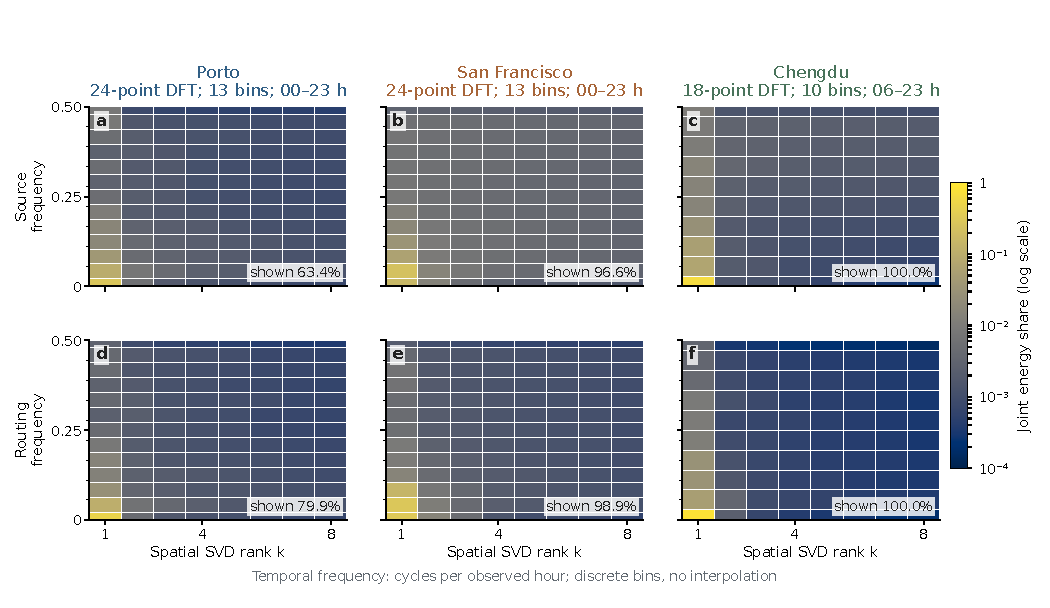
\includegraphics[width=\textwidth]{figures_supp/figS01_joint_spectrum_2d.pdf}
\caption{\textbf{Three-city two-dimensional joint spectra.} Joint energy share over temporal frequency and frequency-specific spatial mode rank for source and full-face routing fields in Porto, San Francisco and Chengdu. The eight-mode display cut is applied after full-spectrum normalization. Porto and San Francisco use 24-point DFTs; Chengdu uses an 18-point observed-block DFT with no night imputation. San Francisco averages frequency energies and within-frequency mode shares separately across TRAIN folds. Spatial rank is not geographical wavelength.}
\label{fig:supp-1}
\end{figure}

\begin{figure}[!htbp]
\centering
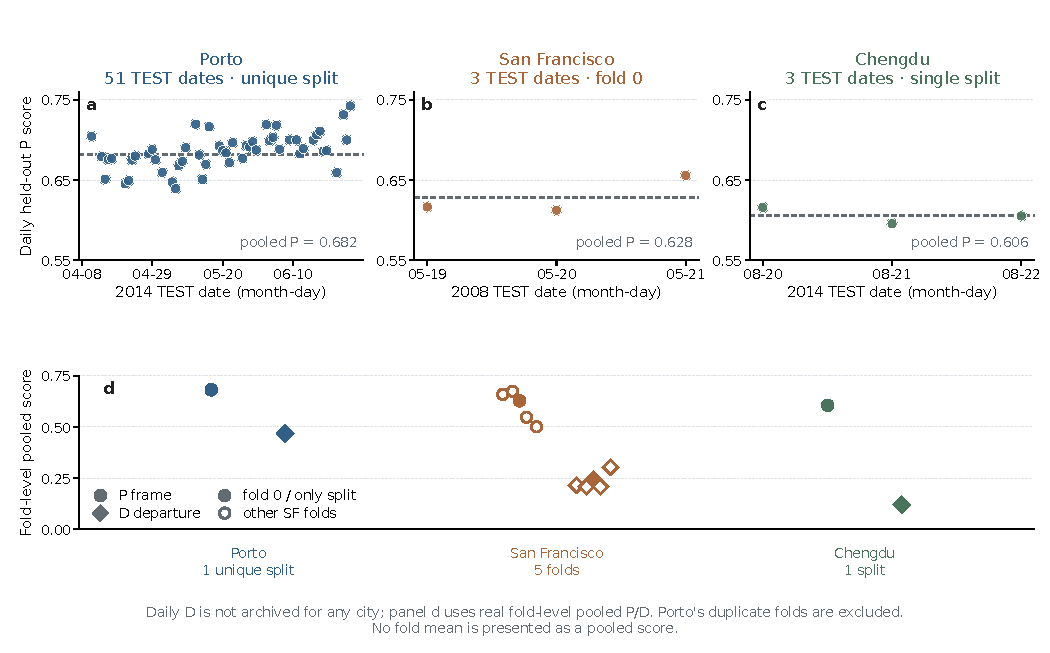
\includegraphics[width=0.95\textwidth]{figures_supp/figS02_heldout_daily_scores.pdf}
\caption{\textbf{Three-city held-out daily P/D scores.} Date-specific P and D values for Porto, San Francisco and Chengdu under the frozen splits in Table~\ref{tab:observation-regimes}. San Francisco retains its five-fold structure; Chengdu has three TEST dates in the continuous-observation protocol. Daily values complement the pooled scores in Table~\ref{tab:crosscity}; their spread is not a paired-date confidence interval.}
\label{fig:supp-2}
\end{figure}

\paragraph{Coherent TRAIN/TEST response.} The frozen P-selected operator is applied without refitting a frequency response. Each date is transformed with the same unitary DFT support as the descriptive spectrum: 24 points in Porto and San Francisco and 18 points in Chengdu. Let $a_m^{(\mathcal S)}$ and $b_m^{(\mathcal S)}$ be observed and predicted routing coefficients averaged over dates in split $\mathcal S\in\{\mathrm{TRAIN},\mathrm{TEST}\}$. For each split and single-sided bin $m$,
\begin{equation}
 \gamma_m^{(\mathcal S)}=\frac{|a_m^{(\mathcal S)*}b_m^{(\mathcal S)}|}{\norm{a_m^{(\mathcal S)}}\norm{b_m^{(\mathcal S)}}},
 \qquad
 \rho_m^{(\mathcal S)}=\frac{\norm{b_m^{(\mathcal S)}}}{\norm{a_m^{(\mathcal S)}}} .
 \label{eq:supp-coherent-response}
\end{equation}
The absolute inner product makes $\gamma_m$ insensitive to a common phase rotation. TRAIN values describe the fit sample; TEST values are held-out. San Francisco summaries are fold means and ranges. These coherent averages complement, rather than replace, observation-level P/D scores. Chengdu evaluates all ten bins $m=0,\ldots,9$, exactly as in its joint spectrum. Figure~\ref{fig:supp-3} displays both splits without treating the TRAIN comparison as independent validation.

\begin{figure}[!htbp]
\centering
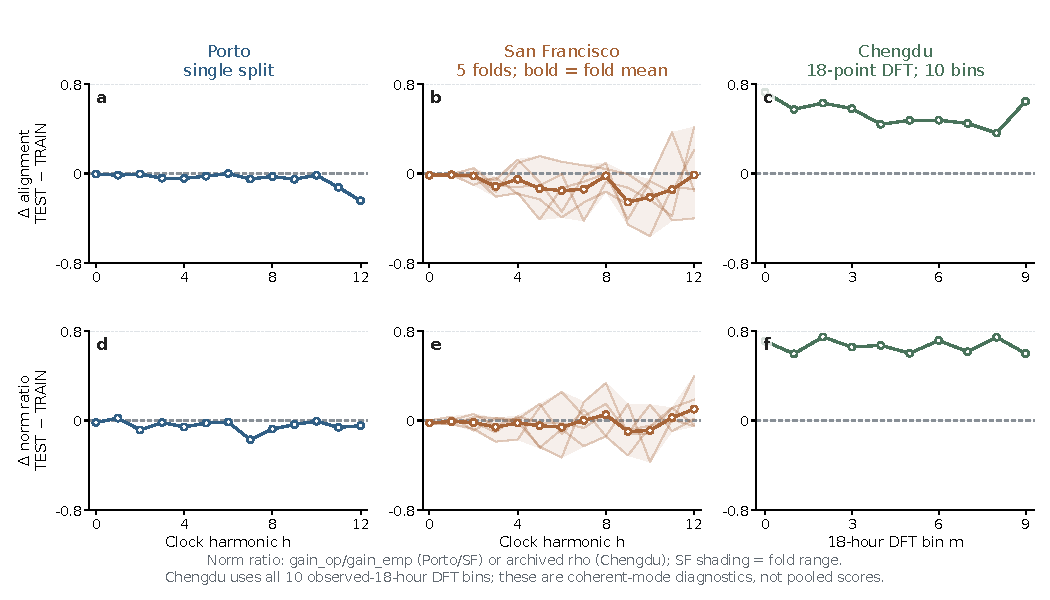
\includegraphics[width=\textwidth]{figures_supp/figS03_coherent_response_train_test.pdf}
\caption{\textbf{Three-city coherent response on TRAIN and TEST.} Direction alignment $\gamma_m$ and predicted-to-observed norm ratio $\rho_m$ for Porto, San Francisco and Chengdu under the frozen P-selected operator. TRAIN values describe the fit sample; TEST values are held-out. San Francisco shows fold means and ranges. Each date uses the same unitary DFT support as the descriptive spectrum; Chengdu evaluates all ten single-sided bins of its 18-point transform. Alignment is insensitive to a common phase rotation.}
\label{fig:supp-3}
\end{figure}

\suppnote{Anisotropy and matched-capacity media}{note:spatial}

\paragraph{Local tensors and axial orientation.} For each regular interior cell, $\Lc$ maps signed face flux to two physical components. Define
\begin{equation}
\begin{aligned}
 \SigC(c)&=\Lc\CR\CR^\top\Lc^\top,\\
 \SigU(c)&=\Lc\UR\UR^\top\Lc^\top,\\
 A(c)&=\begin{cases}
 (\lambda_1(c)-\lambda_2(c))/(\lambda_1(c)+\lambda_2(c)),&\lambda_1(c)+\lambda_2(c)>0,\\
 0,&\lambda_1(c)+\lambda_2(c)=0 .
 \end{cases}
\end{aligned}
\label{eq:supp-local-tensors}
\end{equation}
Here $\lambda_1\ge\lambda_2$ are eigenvalues of the relevant tensor. The principal eigenvector defines an axis $\theta$ modulo $\pi$, not a directed arrow. San Francisco uses per-cell mean anisotropy and a nematic mean of $e^{2i\theta}$ over five folds. Directional coherence is
\begin{equation}
 S_{\mathrm{nem}}=\frac{\left|\sum_cw_c\AC(c)e^{2i\theta_C(c)}\right|}
 {\sum_cw_c\AC(c)},
 \label{eq:supp-nematic}
\end{equation}
with $w_c=1$ or $w_c=\tr\SigC(c)$.

Structural-axis agreement is the joint-anisotropy estimand
\begin{equation}
 G_\theta=\frac{\sum_c\AC(c)\AU(c)\cos[2(\theta_C(c)-\theta_U(c))]}{\sum_c\AC(c)\AU(c)},
 \qquad \AC(c)\AU(c)>0 ,
 \label{eq:supp-axis-agreement}
\end{equation}
on regular interior cells for which both anisotropies are nonzero. Because $\SigC$ uses a unit input metric, we also evaluate the source-covariance-weighted response tensor
\begin{equation}
 \Sigma_{\mathrm{response}}(c)=\Lc\CR\Sigma_{xx}\CR^\top\Lc^\top,
 \label{eq:supp-source-metric}
\end{equation}
with $\Sigma_{xx}$ the TRAIN covariance of source departures. Median anisotropies under this metric are 0.766, 0.926 and 0.765 in Porto, San Francisco and Chengdu, compared with 0.635, 0.651 and 0.705 under the unit metric. Strong local anisotropy persists under source-covariance weighting, indicating that directional selectivity is also pronounced under the realized excitation statistics. This comparison does not establish independence from every possible input metric.

Axis agreement is a separate question because $\CR$ and $\UR$ share the road subspace by construction. We write $K_R=Q\Lambda V^\top$ and replace $Q$ by a Haar-random orthonormal frame $Q_0$ in the road output space, $K_0=Q_0\Lambda V^\top$, preserving the spectrum and input directions. Recomputing $G_\theta$ for 999 draws gives null minima of 0.967, 0.902 and 0.803 and medians of 0.973, 0.911 and 0.808 in Porto, San Francisco and Chengdu. The archived estimates (five-fold consensus for San Francisco), 0.79, 0.79 and 0.76, lie below every null draw, so no observed value exceeds the null (one-sided empirical $p=1.0$ in all three cities). The archived tensors in \path{results/frozen/anisotropy/fo4_fig5_data.npz} and \path{results/frozen/anisotropy/chengdu_anisotropy.npz} are the single primary source for these estimates and for Fig.~\MainRef{fig:road-tests}a--c. Because the rotation requires $K_R$, which is not stored with those tensors, the null is generated by a control refit at the archived $\kappa$ and a single-fold reconstruction (San Francisco fold 0). This control reproduces the archived scale but is not used as an estimate; the reported conclusion uses only the archived estimates against the null quantiles, and the provenance audit records both the archived sources and the control's role. Because the control's own \(G_\theta\) is at least as large as the archived estimate in every city, the comparison is conservative for the reported conclusion. Axis agreement is not distinguishable from the spectrum-matched null and provides no independent evidence of a road-aligned response. We retain only the anisotropy magnitude as an operator property.

On the regular interior grids $\Lc\Lc^\top=2I$, so metric whitening is a no-op and grid anisotropy vanishes there; anisotropic boundary-cell metrics are excluded. An orthogonal road-coordinate rotation leaves the physical tensor unchanged when basis and coefficients are transformed together. Under a rigid physical rotation $Q$,
\begin{equation}
 \SigC(c)\mapsto Q\SigC(c)Q^\top,\qquad v_C(c)\mapsto Qv_C(c),
\end{equation}
while eigenvalues and scalar anisotropy are invariant. The axial vector is covariant, not numerically unchanged in fixed physical coordinates.

\begin{figure}[!htbp]
\centering
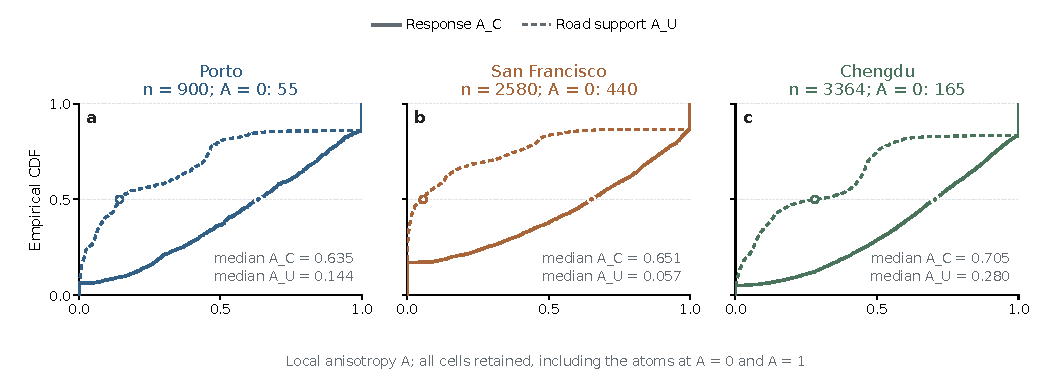
\includegraphics[width=0.72\textwidth]{figS04_anisotropy_distributions.pdf}
\caption{\textbf{Three-city local anisotropy distributions.} Empirical cumulative distribution of $A=(\lambda_1-\lambda_2)/(\lambda_1+\lambda_2)$, with $A=0$ assigned to a zero tensor, over regular interior cells for road support $\AU$ (dashed) and fitted response $\AC$ (solid); circles mark medians. Both curves use the same cells and per-cell definition. Endpoint steps are real atoms: cells without directional energy enter at $A=0$ (5--17\%, identical cell sets for $\AU$ and $\AC$), and one-dimensional tensors enter at $A=1$ (6--16\%). They are not normalization artefacts.}
\label{fig:supp-4}
\end{figure}

\paragraph{Matched-capacity media.} The compared media are a road medium from an external GIS raster, a mobility-inferred medium estimated from TRAIN mobility observations, and a permuted mobility medium. At capacity $R$, each per-face source pattern is averaged over $R$ spatial blocks and passed through the verified mean-1/floor normalization
\begin{equation}
 w^{(R)}_{S,f}=\max\!\left(\frac{\overline W^{(R)}_{S,f}}{\langle\overline W^{(R)}_S\rangle_{\mathrm{interior\ faces}}},\,0.02\right),
 \label{eq:supp-medium-normalization}
\end{equation}
before the archived minimum-energy field lift. Thus $R$ is the nominal number of block values before normalization, not the effective degrees of freedom: mean-1 normalization removes at least one independent degree, and the floor can reduce it further. With $R=1$ every medium is constant, and $R=n_{\mathrm{int}}$ assigns one pre-normalization value per interior face. Permutation preserves the mobility medium's values, partition and nominal block count while permuting its spatial arrangement. Road and mobility media do not have identical information inputs; equal $R$ matches capacity, not information.

The score is computed per held-out date against that date's own target mean and then averaged with equal date weight:
\begin{equation}
 R^2_{\mathrm{cond},d}=1-\frac{\sum_{t\in d}\norm{T_t-\widehat T_t}^2}{\sum_{t\in d}\norm{T_t-\langle T\rangle_d}^2}.
 \label{eq:supp-conditional-score}
\end{equation}
It is an archived date-centred statistic on the raw routing target, not on D's TRAIN-phase departure target, and is distinct from P and D in Eq.~\ref{eq:supp-pd-scores}. Figure~\ref{fig:supp-5} reports gains over the constant $R=1$ medium.

The nested grids are Porto $R=(1,4,16,64,256,1984)$ with block sides $(0,16,8,4,2,1)$; San Francisco $R=(1,3,12,44,176,704,5512)$ with block sides $(0,32,16,8,4,2,1)$; and Chengdu $R=(1,4,16,64,225,900,7080)$ with block sides $(0,32,16,8,4,2,1)$. Side zero denotes the single constant block. The final identity partition gives $R=n_{\mathrm{int}}=(1984,5512,7080)$. San Francisco uses its occupancy-defined channel and per-fold basis; Chengdu has only the archived all-motion channel and uses the frozen per-fold-basis rule on its chronological 10/4/4 split.

\begin{figure}[!htbp]
\centering
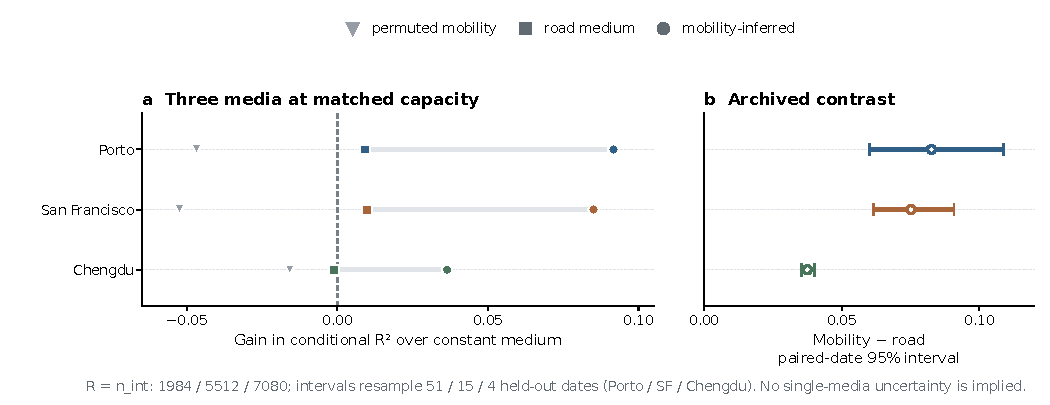
\includegraphics[width=0.68\textwidth]{figS05_matched_capacity.pdf}
\caption{\textbf{Three-city media at matched capacity.} Gain in held-out conditional $R^2$ over the constant $R=1$ medium for the permuted mobility medium, road medium and mobility-inferred medium at $R=n_{\mathrm{int}}$ (1984, 5512 and 7080 nominal pre-normalization block values). The score is the equal-date mean of within-date conditional $R^2$, distinct from P and D. Constant-medium values are 0.613, 0.743 and $-0.030$. Permutation preserves values, partition and nominal block count. Chengdu resamples four alternate-hour dates on a single all-motion channel; its points are small-sample summaries.}
\label{fig:supp-5}
\end{figure}

The matched-capacity modules \texttt{domain\_lib.py} and \texttt{domain\_rankmatched.py} are included in the public export, together with the sweep wrapper. The sweep still requires external aligned fields, date-freeze files and GIS rasters, which are listed with hashes in the data manifest; the archived passing-cell record validates the frozen run and is not a claim that the sweep runs without those inputs.

\suppnote{Baseline and comparison protocols}{note:baselines}

\paragraph{Graph WaveNet.} The completed adaptation \cite{wu2019graphwavenet} estimates the contemporaneous source-to-routing map on the frozen date splits. The implemented \texttt{cc\_lib.anomaly} mask, rather than its misleading ``every row'' docstring, defines a P/FACE score: TRAIN inputs and targets are phase-centred, whereas VAL/TEST inputs and targets remain raw. Predictions are projected with $P_0$, so zero divergence is imposed rather than learned.

The archived loop constructs the network before seeding the training routine, leaving weight initialization uncontrolled. The sealed protocol declares one integer before construction, seeds \texttt{random}, NumPy and PyTorch, and reruns the full four-configuration grid with VAL selection repeated inside every seed. Porto and Chengdu use five seeds; San Francisco uses four seeds common to all five folds. The archived cells remain identifiable as single draws. The final duplicate Porto fold-0 per-date record is authoritative. Graphormer's separate 60-epoch reduced-budget run is excluded from the matched comparison and does not bound its model class.

\paragraph{Gravity and OD overlap.} The doubly constrained gravity model estimates OD flows from TRAIN margins and distance, selecting friction on VAL. Its native common-part-of-commuters score at $4\times4$-cell aggregation is an OD-overlap measure, not a routing $R^2$, and the two are not numerically comparable. Radiation and Deep Gravity were not run because the required population/opportunity or covariate inputs were not supplied; no numerical result is attributed to them \cite{simini2012universal,simini2021deepgravity}.

\paragraph{All-or-nothing loading.} AON uses time-shortest paths with archived road length/speed costs, a 150\,m endpoint-snap threshold, and no congestion equilibrium or capacity calibration. Gravity loading retains the top 150,000 zone pairs under the archived combined-demand rule. A TEST-fitted global amplitude is diagnostic rather than deployable; the fixed-amplitude arm uses $\alpha=1$. Exact-TEST-OD loading has additional demand information and is not a source-only prediction. AON does not stand in for Wardrop user equilibrium \cite{wardrop1952}, which was not run.

Chengdu OD is cut from the corpus occupancy flag as maximal occupied runs, with frozen cleaning breaks (fix gap $>15$\,min, implied speed $>120$\,km\,h$^{-1}$, displacement $>3000$\,m) and retention above 60\,s and 100\,m. It is not inferred from a displacement heuristic. The observed field counts crossings during $[t_k,t_k+3600\,\mathrm{s})$, whereas the loaded field routes every trip whose origin lies in window $k$. Moreover, Chengdu's observed field is marched from every fix while its OD uses occupied runs only; these overlapping but different activity sets are part of the comparison protocol.


\suppsection{Supplementary Results}
\noindent Notes~\ref{note:coupling-results}--\ref{note:structural-results} report held-out coupling, daily scores, coherent response, anisotropy and structural tests. The three-city P-frame physical reconstruction is a qualitative complement to the complete held-out evaluation.

\suppnote{Held-out coupling and baseline results}{note:coupling-results}

\begin{table}[!htbp]
\centering\footnotesize
\caption{\textbf{Three-city P/D/CLIM scores.} P scores the raw target; D scores TRAIN-centred departures; CLIM is the source-free P/ROAD phase clock. Cov.\ is raw routing energy captured by roads. Errors pool held-out observations within each city.}
\label{tab:crosscity}
\setlength{\tabcolsep}{3pt}
\begin{tabular*}{\textwidth}{@{\extracolsep{\fill}}lrrrrrrrrr@{}}
\toprule
 & & & \multicolumn{4}{c}{P} & \multicolumn{3}{c}{D} \\
\cmidrule(lr){4-7}\cmidrule(lr){8-10}
City & Cov. & CLIM & \multicolumn{2}{c}{UrbanFlow} & Ridge & POD & \multicolumn{2}{c}{UrbanFlow} & Ridge \\
\cmidrule(lr){4-5}\cmidrule(lr){8-9}
 & & ROAD & ROAD & FACE & FACE & FACE & ROAD & FACE & FACE \\
\midrule
Porto & 0.904 & 0.472 & 0.682 & 0.607 & 0.701 & 0.701 & 0.468 & 0.411 & 0.504 \\
San Francisco & 0.886 & 0.727 & 0.597 & 0.528 & 0.611 & 0.637 & 0.240 & 0.209 & 0.262 \\
Chengdu & 0.731 & 0.931 & 0.606 & 0.440 & 0.572 & 0.575 & 0.120 & 0.085 & 0.126 \\
\bottomrule
\end{tabular*}
\end{table}

The three focal cities replicate a procedure, not a single operator transferred between cities. Porto has the strongest departure coupling. San Francisco retains positive D scores despite a raw climatology stronger than raw operator reconstruction. Chengdu separates a highly recurrent raw field from weak departure prediction: P/ROAD is 0.606, CLIM is 0.931 and D/ROAD is 0.120. Adding the D departure to the TRAIN climatology gives a full-field gain $\Delta R_I=(1-R_{\rm CLIM})R_D$ of approximately 0.25, 0.07 and 0.008 in Porto, San Francisco and Chengdu. The evidence is therefore hierarchical rather than three equivalent validations: Porto shows a clear conditional relation, San Francisco a weaker but consistent one, and Chengdu a highly recurrent field in which source information adds little beyond the daily pattern.

Paired-date bootstrap intervals for D/ROAD are 0.355--0.528 in Porto, 0.188--0.288 in San Francisco and 0.107--0.142 in Chengdu (10,000 resamples, dates resampled within folds). The source--routing pairing null permutes complete date blocks within TRAIN, VAL and TEST separately and refits the operator in each of 199 draws; null medians are approximately zero, and no Porto or San Francisco draw reaches the observed score (empirical $p=1/200$). Chengdu has only three held-out dates, so its null and interval are descriptive rather than significance tests. Figure~\ref{fig:supp-2} shows the date-resolved values.

Full-face ridge and TRAIN-only POD equal or outperform the road restriction on FACE targets. D/FACE ridge scores are 0.504, 0.262 and 0.126, against road-restricted 0.411, 0.209 and 0.085. Roads therefore supply independently specified, interpretable support rather than the highest linear reconstruction accuracy. Interior-face counts in Porto, San Francisco and Chengdu are 1,984, 5,512 and 7,080; D-frame selected POD ranks are 958, 16 and 64. Table~\ref{tab:crosscity} consistently pools errors rather than averaging fold scores.

\paragraph{Three-city P-frame physical reconstruction.} Figure~\ref{fig:supp-6} visualizes observed and predicted road-supported routing fields using the frozen P estimator with raw TEST inputs and targets. No phase climatology is added and no D departure is substituted. Porto and San Francisco preserve their archived \texttt{picked\_i}/\texttt{picked\_phase} snapshots. Chengdu selects the TEST date whose daily P error is closest to the median daily P error: \texttt{picked\_i=2}, \texttt{picked\_phase=6} (12:00 in the 06--23\,h window), \texttt{picked\_date=16304}. Its pinned-basis export is checked against the frozen $R_{\mathrm P}$. These snapshots are qualitative complements to the complete pooled scores, not additional independent experiments.

\begin{figure}[!htbp]
\centering
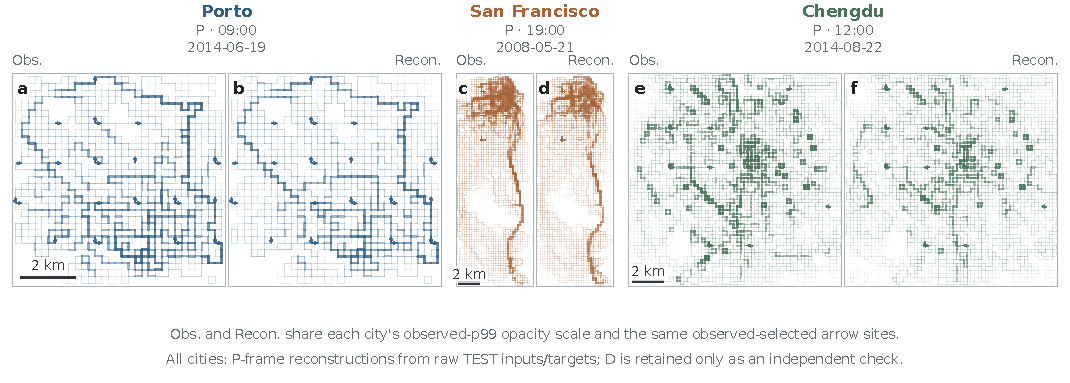
\includegraphics[width=\textwidth]{figS06_heldout_reconstruction.pdf}
\caption{\textbf{Three-city held-out physical reconstruction in the P frame.} Observed and reconstructed road-supported routing fields for Porto, San Francisco and Chengdu, using the frozen P estimator with raw TEST inputs and targets; no phase climatology is added. Porto and San Francisco preserve their archived picked indices and phases. Chengdu uses the TEST date with daily P error closest to the median daily P error, specifically \texttt{picked\_i=2}, \texttt{picked\_phase=6} (12:00), \texttt{picked\_date=16304}, and passes the pinned-basis/frozen-$R_{\mathrm P}$ export check. Observed and predicted panels within a city use identical glyph sites and the observed field's 99th-percentile magnitude scale, with saturation above it; colour scales are city-specific. The maps are qualitative, whereas Table~\ref{tab:crosscity} uses every held-out observation.}
\label{fig:supp-6}
\end{figure}

\paragraph{Neural aggregation.} Seed configuration variability, the archived Porto paired contrast and the sealed seed means are reported in Note~\ref{note:baselines}. Table~\ref{tab:crosscity} and main Table~1 use archived pooled per-date errors, including a San Francisco Graph WaveNet value pooled from its archived per-date records; the sealed San Francisco fold mean is not used for ranking.

\paragraph{Gravity and loading diagnostics.} Native gravity CPC values are 0.525, 0.464 and 0.555. TEST-scaled gravity loading gives 0.136, 0.270 and $8.3\times10^{-5}$; exact-TEST-OD AON gives 0.172, 0.336 and 0.002, with fixed-amplitude values 0.126, $-0.533$ and $-0.565$. These tasks use different inputs and are not source-only accuracy rankings.

Chengdu's OD table contains 1.64\,M TEST trips, of which 1.28\,M remain after snapping. Its strong OD overlap but near-zero loading score is therefore not a ranking of demand quality. The loaded field has cosine 0.04 with the observed field, and destination permutation leaves the loaded field almost unchanged (cosine 0.93--0.94), showing that this pipeline resolves a largely margin-driven pattern. Rebuilding the observed three TEST dates from all fixes reproduces the frozen field at pooled cosine 0.999999. Using occupied runs alone removes 16.3\% of absolute flux, leaves 76\% of energy, and gives pooled cosine 0.929 with the all-fix field. Thus the activity-set difference is real and bounded, but by itself is unlikely to account for the loading mismatch. All loading rows diagnose the implemented demand--registration--loading pipeline rather than attainable performance of traffic assignment as a paradigm.

\suppnote{Joint-spectrum, daily-score and coherent-response results}{note:spectral-results}

The joint field spectra, daily P/D scores and coherent response answer different questions. No operator is refitted for the spectral displays. The coherent comparison uses the same per-date DFT support as the joint spectrum in each city.

\paragraph{Three-city joint spectra.} At the eight-mode display cut in Figure~\ref{fig:supp-1}, source energy coverage is 0.6343, 0.9656 and 1.0000 in Porto, San Francisco and Chengdu, and routing coverage is 0.7989, 0.9892 and 1.0000. Chengdu's complete coverage follows from its eight-TRAIN-date snapshot-rank ceiling and does not demonstrate greater intrinsic low dimensionality. The common logarithmic floor is $10^{-4.5}$; all displayed cells exceed it. Chengdu's time-independent component carries 0.668 of source energy and 0.811 of full-face routing energy. The weighted spectra account for raw-block energy to machine precision; this is a numerical conservation check, not held-out evidence.

\paragraph{Held-out daily P/D scores.} Figure~\ref{fig:supp-2} resolves the pooled entries in Table~\ref{tab:crosscity} by TEST date. Porto has 51 TEST dates, San Francisco has five blocked folds and Chengdu has three TEST dates in the continuous-observation protocol. The daily spread is descriptive: it does not replace the common pooled-error convention and does not supply the missing paired-date interval for the primary D comparison. In particular, Chengdu's three dates are insufficient for a strong date-heterogeneity claim.

\paragraph{Coherent TRAIN/TEST response.} Figure~\ref{fig:supp-3} compares the frozen P-selected operator with observed coherent routing on both TRAIN and TEST. TRAIN panels describe the fit sample and are not independent validation. On TEST, the direction alignments $\gamma_m$ at $m=0$ are 0.978, 0.943 and 0.821 in Porto, San Francisco and Chengdu, respectively; at the first nonzero bin $m=1$ they are 0.935, 0.908 and 0.628. The corresponding norm ratios $\rho_m$ are 0.800, 0.612 and 0.709 at $m=0$, and 0.790, 0.849 and 0.596 at $m=1$. San Francisco values are fold means. Across all ten Chengdu bins, alignment spans 0.474--0.821 and norm ratio spans 0.596--0.747. These results show partial alignment in both direction and magnitude; they do not convert coherent-date averages into observation-level P/D scores.

\begingroup\sloppy
\paragraph{Underpowered Chengdu full-FACE nonlinear exploration.} Figure~\ref{fig:supp-7} reports an exploratory 18-phase A-to-D comparison on the complete FACE target. For each nonlinear arm, $\Delta R^2$ is the mean-date full-FACE error of \texttt{linF} minus that of the arm, so positive values favour the nonlinear arm. The \texttt{quadF} contrast is $-0.005854$ with descriptive 95\% interval $[-0.006105,-0.005661]$; the \texttt{krrF} contrast is $+0.000418$ with interval $[-0.000023,+0.000698]$, which crosses zero.

There are only three TEST dates, and D's all-phase linear design has 144 columns for 144 TRAIN rows and is therefore saturated.

The design is \textbf{underpowered}: these arms neither establish a nonlinear improvement nor support a claim of no nonlinearity.

Full-FACE scores must not be mixed with POD-internal scores. Although 9,999 paired-date bootstrap draws are recorded, three dates provide only 27 ordered date resamples, so the intervals are descriptive rather than confirmatory.

\endgroup

\begin{figure}[!htbp]
\centering
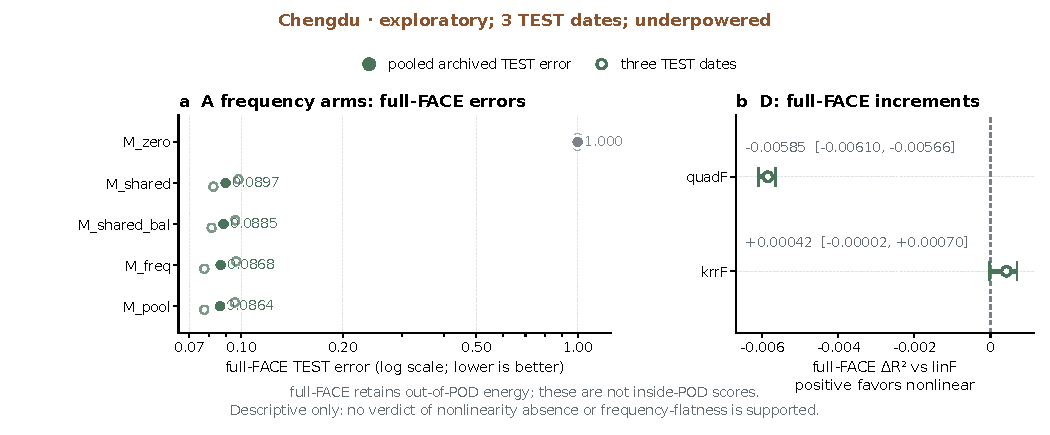
\includegraphics[width=0.74\textwidth]{figures_supp/figS07_nonlinear_exploratory.pdf}
\caption{\textbf{Underpowered exploratory Chengdu full-FACE nonlinear comparison.} Full-FACE $\Delta R^2$ relative to \texttt{linF} for \texttt{quadF} and \texttt{krrF} on the 18-phase A-to-D design, with descriptive 95\% paired-date intervals. \texttt{quadF} gives $-0.005854$ $[-0.006105,-0.005661]$; \texttt{krrF} gives $+0.000418$ $[-0.000023,+0.000698]$. Only three TEST dates are available, and the 144-column linear design saturates the 144 TRAIN rows. The experiment is exploratory and underpowered; it does not demonstrate either the presence or absence of nonlinearity.}
\label{fig:supp-7}
\end{figure}

\suppnote{Three-city anisotropy results}{note:anisotropy-results}

Median response anisotropy is 0.635, 0.651 and 0.705 in Porto, San Francisco and Chengdu, against structural-tensor medians 0.144, 0.057 and 0.280. The response exceeds structural anisotropy at 79.3\% of Porto cells, 71--72\% of San Francisco cells and 72.4\% of Chengdu cells. These are properties of the fitted response on its identified source span, not of the instantaneous flow distribution. Figure~\ref{fig:supp-4} shows the full distributions behind these medians. Its zero-response atoms are distinct from low but nonzero anisotropy, and its rank-one atoms explain the vertical approach at $A=1$.

Strong local anisotropy does not imply one city-wide preferred direction. Unweighted nematic coherence is 0.087 in Porto, 0.21--0.22 across San Francisco folds and 0.057 in Chengdu. Principal axes vary across space rather than collapsing onto one compass orientation.

Using the joint $\AC\AU$-weighted estimand in Eq.~\ref{eq:supp-axis-agreement}, structural-axis similarity is 0.79, 0.79 and 0.76 in Porto, San Francisco and Chengdu. San Francisco's anisotropy map is reproducible across five folds, with mean pairwise spatial correlation 0.984 (range 0.974--0.991) and anisotropy-weighted nematic axis agreement 0.993. The invariance checks concern scalar anisotropy and covariant axial/tensor transformations as specified in Note~\ref{note:spatial}; they do not imply an axis that remains numerically unchanged under a rigid physical rotation.

\suppnote{Road specificity and matched-capacity structural results}{note:structural-results}

\paragraph{Rank-matched subspace specificity.} The structural test uses each city's full aligned observation pool, not the held-out P/D pool. Full-pool road captures are 0.900, 0.900 and 0.731 in Porto, San Francisco and Chengdu. Every one of the 999 random conservation-compatible subspaces leaves more routing energy uncaptured than the real road subspace (0/999 at least as good, empirical $p=1/1000$). The excess $\Delta E=E_{\mathrm{null}}-E_{\mathrm{road}}$ ranges from 0.23 to 0.30 in Porto, 0.28 to 0.33 in San Francisco and 0.09 to 0.15 in Chengdu. This is a null distribution, not a confidence interval. The ambient $\ker D$ and rank are fixed while the random subspaces vary; the result concerns representation specificity and does not show that a source predicts the state within the road space.

\paragraph{Matched-capacity media.} At $R=n_{\mathrm{int}}=(1984,5512,7080)$ nominal pre-normalization block values, the constant-medium held-out $\Rcond$ values are 0.613, 0.743 and $-0.030$. Road-medium gains over that reference are 0.009, 0.010 and $-0.001$; mobility-inferred gains are 0.092, 0.085 and 0.036; and permuted-mobility-medium gains are $-0.047$, $-0.052$ and $-0.016$. The paired mobility-minus-road differences are 0.083 in Porto (95\% interval 0.060--0.109), 0.075 in San Francisco (0.062--0.091) and 0.038 in Chengdu (0.035--0.040). Figure~\ref{fig:supp-5} shows all three media at this capacity.

The comparison matches capacity and estimator, not information: the road pattern is an external GIS raster, whereas the mobility-inferred pattern is estimated from TRAIN mobility. Both use the same nominal block capacity under the same normalization. Permuting the mobility medium's spatial arrangement preserves its values, partition and nominal block count and removes the gain. Chengdu uses one all-motion channel, a frozen per-fold basis and four held-out alternate-hour dates; its interval resamples only those dates. The design cannot separate the influence of date count, delivery phase and channel, and the four-date interval is only a descriptive summary, not the 14-date P/D experiment.

Together, the two tests show that the road-induced subspace is not generic under the stated rank-matched null, while the road-only medium does not match the mobility-inferred medium under this estimator and information regime. They do not show that road geometry lacks physical meaning, that all alternative road structures have been tested, or that source-only closure has been achieved. The source files, real $R$ grids and missing-module definition gap are listed in Notes~\ref{note:spatial} and \ref{note:reproducibility}.

\begin{table}[!htbp]
\centering\small
\caption{\textbf{Rank-matched and matched-capacity structural controls.} Full results from the former main Fig.~4d--e. The rank-matched test uses the full aligned observation pool; the matched-capacity test uses the date-centred conditional score.}
\label{tab:supp-structural-controls}
\begin{tabular}{lccc}
\toprule
Control & Porto & San Francisco & Chengdu \\
\midrule
Road capture, full pool & 0.900 & 0.900 & 0.731 \\
Rank-matched nulls at least as good & 0/999 & 0/999 & 0/999 \\
Excess $\Delta E$ range & 0.23--0.30 & 0.28--0.33 & 0.09--0.15 \\
Road-medium gain at $R=n_{\rm int}$ & 0.009 & 0.010 & $-0.001$ \\
Mobility-medium gain at $R=n_{\rm int}$ & 0.092 & 0.085 & 0.036 \\
Paired mobility $-$ road [95\%] & 0.083 [0.060, 0.109] & 0.075 [0.062, 0.091] & 0.038 [0.035, 0.040] \\
\bottomrule
\end{tabular}
\end{table}

\paragraph{Road-modulated operator in the FACE-departure frame.} The road-medium test uses a different target from the rank-matched and matched-capacity tests above: the full divergence-free departure $\delta F_t^\circ$, scored by Eq.~\ref{eq:supp-facedep}. The frozen road operator reaches 0.0619 in Porto, 0.0649 in San Francisco and 0.0039 in Chengdu. These values are not comparable with the P/FACE entries of Supplementary Table~\ref{tab:supp-pface-loading} or the ROAD-support D scores; the unrestricted FACE ridge on the same rows reaches 0.5044, 0.2582 and 0.1258. A uniform medium gives a response at floating-point zero, and face permutation or a $90^\circ$/$270^\circ$ rotation of the medium collapses the held-out score to at most 0.005. The operator's selected spectral order is at the pre-registered grid boundary in all three cities.

\begin{table}[!htbp]
\centering\small
\caption{\textbf{Road-medium contrast in the FACE-departure frame.} Held-out $R^2$ for the road-modulated operator, directionally matched Null-1 and coarse-matched Null-2; ``best'' is the highest accepted draw. The unrestricted FACE ridge is shown for scale only. Dashes mark families that could not be constructed under the frozen criteria.}
\label{tab:supp-roadmedium}
\begin{tabular}{lccc}
\toprule
Score & Porto & San Francisco & Chengdu \\
\midrule
Road operator & 0.0619 & 0.0649 & 0.0039 \\
Null-1 mean & 0.0011 & 0.0040 & 0.0003 \\
Null-1 best & 0.0145 & 0.0273 & 0.0018 \\
Null-2 mean & 0.0046 & -- & 0.0010 \\
Null-2 best & 0.0259 & -- & 0.0019 \\
FACE ridge (scale) & 0.5044 & 0.2582 & 0.1258 \\
\bottomrule
\end{tabular}
\end{table}

The nominal draw counts are 499/199/199 for Null-1 and 99/--/49 for Null-2 in Porto/San Francisco/Chengdu; participation-ratio effective sizes are 148/93/175 and 5.6/--/12.4. The corresponding Monte-Carlo floors are 0.002/0.005/0.005 and 0.010/--/0.020.

A directionally matched non-road medium, preserving the exact weight multiset and 26 spatial statistics within the frozen tolerances, does not reproduce the road score: 0 of 499 accepted draws in Porto and 0 of 199 in San Francisco and Chengdu reach it. The best draws reach 23\%, 42\% and 47\% of the road value. In Porto and Chengdu, coarse matching raises the surrogate mean by factors of 4.1 and 3.6 over Null-1, respectively, but the road remains 2.4 and 2.1 times the best coarse draw. San Francisco has no accepted coarse-matched draw (0 of 199), so its evidence supports directional but not fine-scale specificity. The coarse families contain only about six and twelve effective independent configurations, and their tail estimates sit at the design floor; they bound the constructed family rather than calibrating a tail probability.

\paragraph{Road prior beyond a learned learner.} Used as a prior under an equal-capacity residual ridge, the road operator raises held-out $R^2$ by 0.0116 in Porto, 0.0207 in San Francisco and 0.0023 in Chengdu. These are relative residual-SSE reductions of 2.27\%, 2.65\% and 0.26\%, respectively. The 20 directionally matched priors change held-out $R^2$ by between $-0.0013$ and $+0.0003$. The road increment is positive on every Porto TEST date and in three of four blocked Porto folds; the fourth, highest-energy block is negative. The increment is largest when TRAIN is reduced, consistent with a prior that substitutes for data, and the Porto learner sits at the top of its rank grid, so the measured increment is a lower bound in a saturated regime. The prior-only score is still far below the learned model, and the learned correction has no reproducible response direction across TRAIN halves (median cosine 0.20--0.46). The evidence is for an informative structural prior, not an identified learned operator.


\suppsection{Supplementary Reproducibility}
\suppnote{Artifact map and reproducibility}{note:reproducibility}

Table~\ref{tab:artifact-map} separates frozen-score recomputation, figure rebuilding and incomplete raw/training exports. All paths are repository-relative. A file's presence does not imply that an end-to-end raw-trajectory rebuild is possible, and missing modules or per-run outputs are stated rather than replaced by inferred definitions.

\begin{table}[!htbp]
\centering\scriptsize
\caption{\textbf{Artifact and reproducibility map.} Paths are relative to the repository root. The status column distinguishes archived evidence from entry points runnable in the present export.}
\label{tab:artifact-map}
\setlength{\tabcolsep}{3pt}
\begin{tabular*}{\textwidth}{@{\extracolsep{\fill}}>{\raggedright\arraybackslash}p{2.0cm}>{\raggedright\arraybackslash}p{7.15cm}>{\raggedright\arraybackslash}p{6.1cm}@{}}
\toprule
Result family & Source artifacts and code & Reproduction status or limitation \\
\midrule
P/D/CLIM and linear controls & \path{reports/mainstream_mobility_comparison/crosscity_results.csv}; \path{reports/mainstream_mobility_comparison/results/s1/*.json}; \path{reports/mainstream_mobility_comparison/scripts/s1_crosscity.py} & Frozen per-fold objects and pooled scores; no primary-D interval or pairing-null result is supplied. \\
Daily scores and coherent response & \path{reports/mainstream_mobility_comparison/results/s1/*.json}; \path{reports/spatiotemporal_constitutive_spectra/results/obj_*.json}; \path{reports/threecity_redesign/results/chengdu_response18.npz} & Frozen date-level P/D diagnostics and coherent objects; Chengdu uses all ten 18-point DFT bins, and San Francisco fold aggregation remains distinct from pooled scoring. The present Chengdu response file contains TEST only; a TRAIN display requires a same-protocol TRAIN export rather than inference from TEST. \\
Three-city physical reconstruction & \path{crosscity_sample_complexity/artifacts/routing_snapshot_Porto.npz}; \path{crosscity_sample_complexity/artifacts/routing_snapshot_SF.npz}; \path{crosscity_sample_complexity/artifacts/routing_snapshot_meta.json}; \path{reports/threecity_redesign/results/chengdu_snapshot18.npz}; \path{reports/threecity_redesign/results/chengdu_frozen_response_manifest.json}; \path{reports/threecity_redesign/scripts/chengdu_frozen_response.py} & All three snapshots use the P estimator with raw TEST inputs and targets. Chengdu passes pinned-basis and frozen-$R_{\mathrm P}$ checks and archives \texttt{picked\_i=2}, \texttt{picked\_phase=6}, \texttt{picked\_date=16304}. Qualitative snapshots do not replace complete held-out scores. \\
Chengdu nonlinear exploration & \path{reports/chengdu_nonlinear_exploratory/config.json}; \path{reports/chengdu_nonlinear_exploratory/scripts/run_experiment.py}; \path{reports/chengdu_nonlinear_exploratory/results/chengdu_nonlinear_exploratory.json}; \path{reports/chengdu_nonlinear_exploratory/results/validation.json} & Sixteen validation checks pass. The 18-phase full-FACE A-to-D experiment is underpowered: three TEST dates, 144 columns/144 TRAIN rows, and only 27 ordered date resamples. It supports neither nonlinear improvement nor absence of nonlinearity; full-FACE and POD-internal scores remain distinct. \\
Archived neural draw & \path{reports/deep_baseline_training_record/MANIFEST.csv}; \path{reports/deep_baseline_training_record/artifacts/_perdate.jsonl}; \path{reports/deep_baseline_training_record/artifacts/modern_results_all.csv}; \path{reports/deep_baseline_training_record/scripts/run_modern.py} & Twenty copied files were MD5-checked with no mismatch. Large predictions, Jacobians and logs are not included; scripts require legacy-root configuration. \\
Sealed Graph WaveNet & \path{reports/table_fill_chengdu/README.md}; \path{reports/table_fill_chengdu/scripts/gwnet_fixed.py}; \path{reports/table_fill_chengdu/scripts/seal_proof.py} & Seed means, ranges and initialization proof are summarized; complete sealed per-run JSON outputs are not present in this export. San Francisco remains fold-mean aggregation. \\
Gravity and AON & \path{reports/mainstream_mobility_comparison/results/s3/}; \path{reports/mainstream_mobility_comparison/results/s4/}; \path{reports/table_fill_chengdu/README.md} & Archived JSON artifacts and the Chengdu collated record support the three-city scores; loading tasks remain distinct from source-only inference. \\
Joint three-city spectrum & \path{reports/threecity_joint_spectrum/manuscript_revision/verified_joint.npz}; \path{reports/threecity_joint_spectrum/manuscript_revision/audit.json}; \path{reports/threecity_joint_spectrum/manuscript_revision/redraw_joint_spectrum.py} & Weighted Parseval display, source hashes and render checks are archived. Figure rebuilding does not refit an operator. \\
Anisotropy & \path{full_operator_spatial_anisotropy/results/fo4_fig5_data.npz}; \path{results/kr_response_characteristics/}; \path{reports/threecity_figure5_revision/results/chengdu_anisotropy_summary.json} & Frozen arrays and Chengdu D/P sensitivity records support the three-city maps and distributions. \\
Structural null & \path{final_ablation/results/partA_topology.json}; \path{reports/threecity_figure5_revision/results/partA_chengdu.json}; \path{reports/threecity_figure5_revision/scripts/cd_partA_null.py} & 999 draws per city; Chengdu includes a Porto control rerun to machine precision. Full-pool representation test only. \\
Matched-capacity media & \path{benchmark/scripts/bench_lib.py}; \path{benchmark/domain_rankmatched_results.csv}; \path{benchmark/domain_rankmatched_pairwise.csv}; \path{reports/threecity_figure5_revision/results/partF_summary.json}; \path{reports/threecity_figure5_revision/scripts/cd_partF_sweep.py} & The passing-cell record is not a current-export run. \texttt{domain\_rankmatched.py} and \texttt{domain\_lib.py} are absent, the wrapper retains a legacy absolute root, and required aligned fields, date-freeze files and GIS rasters are unavailable. Only frozen results and figure rebuilding are supported. \\
Canonical supplementary figures & \path{paper/merged_manuscript/figures_supp/README.md}; \path{reports/threecity_figure5_revision/scripts/fig5_redesign.py}; manuscript figure scripts & Seven canonical PDFs map one-to-one to Figures~\ref{fig:supp-1}--\ref{fig:supp-7}; figure rebuilding is distinct from recomputing the experiments. \\
\bottomrule
\end{tabular*}
\end{table}

\paragraph{Deep-baseline record.} The archived scoring chain is \texttt{run\_modern.py} $\rightarrow$ \texttt{bmlib.anomalies} $\rightarrow$ \texttt{cc\_lib.anomaly}. Only TRAIN rows are phase-centred by the called implementation, leaving VAL/TEST raw. Deduplicating Porto GWNET fold 0 by retaining the final authoritative per-date record gives an archived single draw of 0.4970176832 in Porto; this is not the sealed seed mean. Graphormer's 60-epoch budget and incomplete fold-level prediction-file export remain disclosed. Per-date error records exist for all scored archived folds, but zero-divergence residuals follow from projection and are not learned conservation.

\paragraph{Release scope and unresolved checks.} The public export is intended to separate figure rebuilding from frozen products, core-score recomputation and end-to-end raw-trajectory reconstruction. It contains no individual-level trajectory records. Large prediction files, unavailable original training artifacts, the missing matched-capacity modules named above, and incomplete sealed per-run outputs must not be represented as included. Raw-data redistribution requirements, OSM snapshot/version and per-artifact licence notices remain release checks (Note~\ref{note:data}). Public repository location: \repositorylocation.


\FloatBarrier
{\footnotesize\makeatletter\def\@listi{\leftmargin\leftmargini \parsep 0\p@ \topsep 2\p@ \itemsep 0\p@}\let\@listI\@listi\makeatother
\bibliographystyle{unsrt}
\bibliography{refs}
}
\end{document}
